\documentclass{beamer}

\usepackage{amsmath}

\usetheme{AnnArbor}
\usecolortheme{crane}
\usefonttheme[onlymath]{serif}

\title{Deep Learning - Foundations and Concepts}
\subtitle{Chapter 1. The Deep Learning Revolution}
\author{nonlineark@github}
\date{\today}

\begin{document}

\begin{frame}
    \titlepage
\end{frame}

\begin{frame}
    \frametitle{Outline}
    \tableofcontents
\end{frame}

\section{The Impact of Deep Learning}

\begin{frame}
    \frametitle{Medical diagnosis}
    \begin{figure}
        \caption{Examples of skin lesions}
        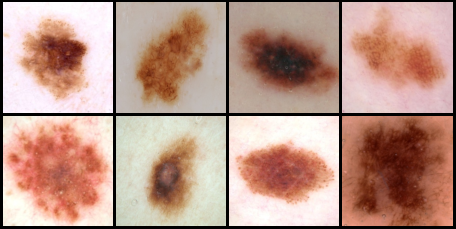
\includegraphics{Figure_1.pdf}
    \end{figure}
\end{frame}

\begin{frame}
    \frametitle{Medical diagnosis}
    \begin{itemize}
        \item Training set: 129K lesion images labelled as either malignant or benign.
        \item Training:
        \begin{itemize}
            \item A deep neural network with 25M adjustable parameters.
            \item First trained on a much larger data set of 1.28M images of everyday objects, and then \emph{fine-tuned} on the data set of lesion images.
            \item This is an example of \emph{transfer learning}.
        \end{itemize}
        \item This is an example of a \emph{supervised learning} problem.
        \item This is also an example of a \emph{classification} problem, compare with \emph{regression} problems where the output consists of one or more continuous variables.
    \end{itemize}
\end{frame}

\begin{frame}
    \frametitle{Protein structure}
    \begin{figure}
        \caption{3D shape of a protein called T1044/6VR4}
        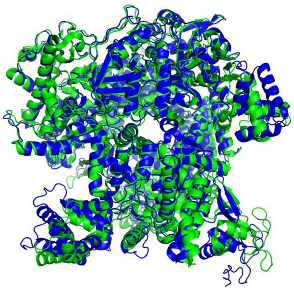
\includegraphics{Figure_2.pdf}
    \end{figure}
\end{frame}

\begin{frame}
    \frametitle{Image synthesis}
    \begin{figure}
        \caption{Synthetic face images}
        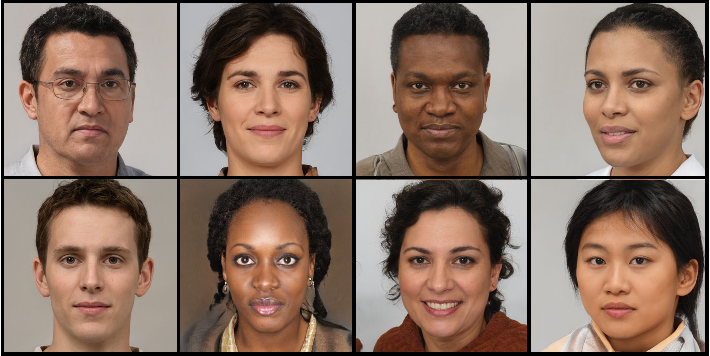
\includegraphics{Figure_3.pdf}
    \end{figure}
\end{frame}

\begin{frame}
    \frametitle{Large language models}
    \begin{itemize}
        \item \emph{Autoregressive} language models can generate language as output.
        \item This is an example of \emph{self-supervised learning}.
    \end{itemize}
\end{frame}

\section{A Tutorial Example}

\begin{frame}
    \frametitle{Synthetic data}
    \begin{figure}
        \caption{Plot of a training data set}
        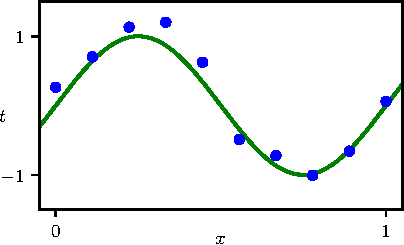
\includegraphics{Figure_4.pdf}
    \end{figure}
\end{frame}

\begin{frame}
    \frametitle{Synthetic data}
    \begin{block}{Problem}
        Given input variables $x=\begin{pmatrix}
            x_{1} \\
            x_{2} \\
            \vdots \\
            x_{N}
        \end{pmatrix}$ and target variables $t=\begin{pmatrix}
            t_{1} \\
            t_{2} \\
            \vdots \\
            t_{N}
        \end{pmatrix}$, predict the value of $\hat{t}$ for some new value of $\hat{x}$.
    \end{block}
\end{frame}

\begin{frame}
    \frametitle{Linear models and error function}
    \begin{block}{Problem'}
        Find $w=\begin{pmatrix}
            w_{0} \\
            w_{1} \\
            \vdots \\
            w_{M}
        \end{pmatrix}$, such that the linear model $y(x;w)=\sum_{j=0}^{M}w_{j}x^{j}$ has the smallest error, as defined by $E(w)=\frac{1}{2}\sum_{n=1}^{N}(y(x_{n};w)-t_{n})^{2}$.
    \end{block}
\end{frame}

\begin{frame}
    \frametitle{Linear models and error function}
    Differentiate $E(w)$, we see that:
    \begin{equation*}
        \begin{split}
            DE(w)&=\sum_{n=1}^{N}(y(x_{n};w)-t_{n})X_{n}^{T} \\
            &=\sum_{n=1}^{N}w^{T}X_{n}X_{n}^{T}-\sum_{n=1}^{N}t_{n}X_{n}^{T} \\
            &=w^{T}X^{T}X-t^{T}X
        \end{split}
    \end{equation*}
    where $X_{n}=\begin{pmatrix}
        1 \\
        x_{n} \\
        \vdots \\
        x_{n}^{M}
    \end{pmatrix}$, and $X=\begin{pmatrix}
        X_{1}&X_{2}&\hdots&X_{N}
    \end{pmatrix}^{T}$.
    
    Let $DE(w^{*})=0$, we have $w^{*}=(X^{T}X)^{-1}X^{T}t$.
\end{frame}

\begin{frame}
    \frametitle{Model complexity and regularization}
    \begin{figure}
        \caption{Root-mean-square error vs. $M$}
        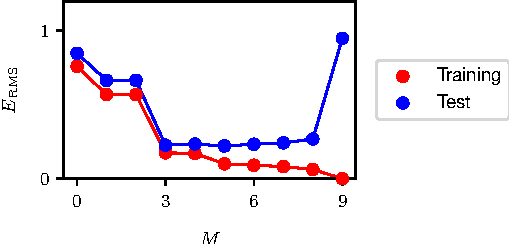
\includegraphics{Figure_7.pdf}
    \end{figure}
\end{frame}

\begin{frame}
    \frametitle{Model complexity and regularization}
    There are several ways to control the \emph{over-fitting} phenomenon:
    \begin{itemize}
        \item Limit the number of parameters in a model according to the size of the available training set.
        \item \emph{Regularization}: Add a penalty term to the error function to discourage the coefficients from having large magnitudes.
    \end{itemize}
    \begin{equation*}
        \tilde{E}(w)=\frac{1}{2}\sum_{n=1}^{N}(y(x_{n};w)-t_{n})^{2}+\frac{\lambda}{2}||w||^{2}
    \end{equation*}
\end{frame}

\begin{frame}
    \frametitle{Model complexity and regularization}
    \begin{figure}
        \caption{Root-mean-square error vs. $\log\lambda$}
        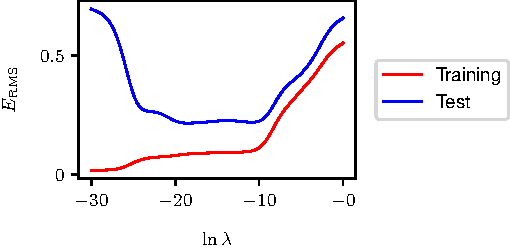
\includegraphics{Figure_10.pdf}
    \end{figure}
\end{frame}

\begin{frame}
    \frametitle{Model selection}
    \begin{itemize}
        \item \emph{Hyperparameter}: Values are fixed during the minimization of the error function, e.g., $M$ and $\lambda$.
        \item Training set, \emph{validation set} and \emph{test set}:
        \begin{itemize}
            \item Training set: Determine the coefficients $w$.
            \item Validation set: Select the model having the lowest error.
            \item Test set: Sometimes over-fitting to the validation set can occur, keep aside a third test set to evaluate the performance of the selected model.
        \end{itemize}
        \item \emph{Cross-validation}
    \end{itemize}
\end{frame}

\end{document}